\section{Algorithm/Scheme for solving the coupled equations}
In this section, the scheme to solve the coupled Poisson's,
Nernst-Planck and Navier-Stokes equations is described. The
dependencies between the equations are shown in
fig. \ref{fig:coupling}.

Following an initialisation of
the velocity field and charge density, an iteration in time is
performed. At each time step, a potential and electric field is
computed by solving Poisson's equation for the present charge
density. This is followed by updating the charge density from the new
potential and then the velocity field is updated with the prescence of
a force related to the charge density. The main ingredients in the
iterative algorithm are shown in fig. \ref{fig:lbm:full_algo}. 

\begin{figure}
\begin{center}
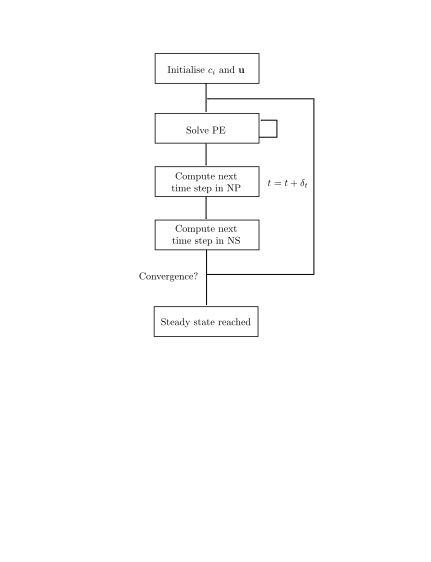
\includegraphics[width=0.4\textwidth]{fig/full_algorithm.pdf}
\end{center}
\caption{Flow scheme of the algorithm for solving the coupled equations.}
\label{fig:lbm:full_algo}
\end{figure}
